\documentclass[conference]{IEEEtran}
\IEEEoverridecommandlockouts
\usepackage{cite}
\usepackage{amsmath,amssymb,amsfonts,amsthm}
\usepackage{graphicx}
\usepackage{textcomp}
\usepackage{booktabs}
\usepackage{multirow}
\usepackage{xcolor}
\usepackage{tikz}
\usetikzlibrary{arrows.meta,positioning,fit,calc}
\usepackage{algorithm}
\usepackage{algpseudocode}
\usepackage[hidelinks]{hyperref}
\usepackage{url}
\newtheorem{definition}{Definition}
\newtheorem{proposition}{Proposition}
\newtheorem{remark}{Remark}
\newcommand{\Vb}{\mathsf{V}}
\newcommand{\Pb}{\mathsf{P}}
\newcommand{\RQ}[1]{\textbf{RQ#1}}
\algrenewcommand\algorithmicrequire{\textbf{Input:}}
\algrenewcommand\algorithmicensure{\textbf{Output:}}

\begin{document}

\title{Fidelity Cores: How Much Configuration Does a\\ Security Service Twin Actually Need?}

\author{\IEEEauthorblockN{Author Name(s)}
\IEEEauthorblockA{\textit{Department, Organization}\\
City, Country \\
email@organization.org}}

\maketitle

\begin{abstract}
Security digital twins promise a safe place to test claims about production services, but a twin is only as trustworthy as the configuration it carries. We ask which part of a configuration actually decides a security verdict, and what a twin gets wrong when it mirrors only some of it. We define \emph{fidelity cores} (minimal directive sets that reproduce a verdict), \emph{pivots} (directives whose removal alone flips it) and \emph{guard sets} (keys whose edits warrant re-emulation), and prove when guard-based synchronization is exact. We measured them on real Redis, PostgreSQL, Nginx and OpenSSH servers and 16 pinned builds. The data comprise 240 seeded configurations with 14,400 drift edits, 1,092 public configuration files and 426 real commits, about 60,000 server runs in all. Verdicts were concentrated: no core exceeded two directives, synthetic or public. Yet partial twins were fragile, wrong 6.6\% of the time with 90\% of directives mirrored at random, because 39\% of pivots lay outside the cores. Guard sets learned only from synthetic data reproduced all 450 tested public verdicts while exporting 24\% of Redis and 12\% of OpenSSH directives. On real commits they needed 137 re-emulations instead of 426, catching all 19 verdict flips. Two effects hidden by version numbers were large. The official Redis 7.0.15 container defaults protected mode off where the Ubuntu build defaults it on, and a platform default profile misjudged 22\% of public sshd configurations even at full synchronization. A careful static analyzer still disagreed with the servers on rare, documented semantic corners.
\end{abstract}

\begin{IEEEkeywords}
digital twin, configuration fidelity, security validation, delta debugging, configuration drift, service emulation, misconfiguration
\end{IEEEkeywords}

\section{Introduction}

A configuration file is a strange object to copy. Most of it is housekeeping: buffer sizes, log formats, keep-alive timers. A few lines, sometimes one, decide whether a database answers a stranger. A security digital twin that copies everything is faithful, but expensive to build, to keep current and to trust with customer data. A twin that copies too little can be confidently wrong. Our earlier platform for configuration-synchronized service twins~\cite{dtplatform} made the second danger concrete: twins rendered from default settings reached an F1 score of only 0.40 on a declared benchmark, while synchronized twins were correct on every conclusive run. That result settled \emph{whether} configuration matters. It did not say \emph{how much} of it matters, or \emph{which} part.

These questions have practical weight. Every directive an agent exports widens what a shared control plane holds about a customer. Every configuration change triggers re-emulation if the platform watches content hashes, and re-emulation is the most expensive step in the pipeline. When a twin reports a weakness, an operator wants to know which lines are responsible and which lines are quietly holding the line. All three needs turn on the same unknown: the relationship between individual directives and a security verdict.

Fig.~\ref{fig:example} shows why the relationship is not obvious. The Nginx configuration has a server-wide \texttt{deny all} and HTTP basic authentication, two lines any reviewer would mark as protective. Yet \texttt{/admin/} is reachable without credentials, because \texttt{satisfy any} lets a matching \texttt{allow} rule stand in for authentication. The lines that decide the outcome are not the lines that look important, and a twin that drops either of them reports the wrong answer.

\begin{figure}[t]
\centering
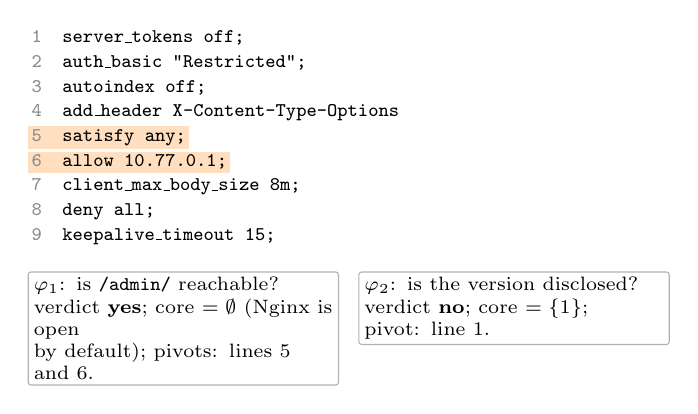
\begin{tikzpicture}[font=\scriptsize\ttfamily, every node/.style={inner sep=1.2pt, anchor=west}]
\def\dy{3.15mm}
\node at (0,0)        {\textcolor{black!45}{1}~~server\_tokens off;};
\node at (0,-1*\dy)   {\textcolor{black!45}{2}~~auth\_basic "Restricted";};
\node at (0,-2*\dy)   {\textcolor{black!45}{3}~~autoindex off;};
\node at (0,-3*\dy)   {\textcolor{black!45}{4}~~add\_header X-Content-Type-Options};
\node[fill=orange!25] at (0,-4*\dy) {\textcolor{black!45}{5}~~satisfy any;};
\node[fill=orange!25] at (0,-5*\dy) {\textcolor{black!45}{6}~~allow 10.77.0.1;};
\node at (0,-6*\dy)   {\textcolor{black!45}{7}~~client\_max\_body\_size 8m;};
\node at (0,-7*\dy)   {\textcolor{black!45}{8}~~deny all;};
\node at (0,-8*\dy)   {\textcolor{black!45}{9}~~keepalive\_timeout 15;};
\node[font=\scriptsize\rmfamily, text width=38mm, align=left, anchor=north west, draw=black!30, rounded corners=1pt, inner sep=2pt] at (0,-9.4*\dy) {$\varphi_1$: is \texttt{/admin/} reachable?\\ verdict \textbf{yes}; core $=\emptyset$ (Nginx is open\\ by default); pivots: lines 5 and 6.};
\node[font=\scriptsize\rmfamily, text width=38mm, align=left, anchor=north west, draw=black!30, rounded corners=1pt, inner sep=2pt] at (42mm,-9.4*\dy) {$\varphi_2$: is the version disclosed?\\ verdict \textbf{no}; core $=\{1\}$;\\ pivot: line 1.};
\end{tikzpicture}
\caption{A configuration from our synthetic corpus, with block structure flattened for space. Shaded lines are \emph{pivots} for $\varphi_1$: removing either one makes the twin report ``closed''. The protective-looking lines 2 and 8 can each be removed without changing the verdict.}
\label{fig:example}
\end{figure}

This paper studies the relationship between directives and verdicts directly, on unmodified servers, through seven questions:
\begin{itemize}
\item[\RQ{1}] How does verdict accuracy degrade when a twin mirrors only part of a configuration?
\item[\RQ{2}] How large are minimal verdict-preserving subsets, are they unique, and do they contain the directives that are individually necessary?
\item[\RQ{3}] Can a twin be built from a learned set of keys, and does that set transfer from synthetic to real configurations?
\item[\RQ{4}] When a configuration drifts, which policy decides best when to re-emulate?
\item[\RQ{5}] How much do the server version and the build of a version change verdicts?
\item[\RQ{6}] Do the findings hold on configurations from public repositories and their histories?
\item[\RQ{7}] Could a careful static analyzer replace the twin?
\end{itemize}

\noindent Our contributions are:
\begin{itemize}
\item \textbf{Concepts.} We define verdict-relative fidelity for service twins: fidelity curves, fidelity cores (sufficiency), pivots (necessity) and key guard sets. Two conditions, key locality and base silence, make selective synchronization and key-guarded re-emulation provably exact (Section~\ref{sec:concepts}).
\item \textbf{A measurement harness} that renders configurations onto real servers and 16 pinned builds, and probes each over the wire with stock clients (Section~\ref{sec:design}).
\item \textbf{Three corpora}: 240 seeded configurations with 14,400 drift edits; 1,092 distinct public configuration files; and 216 public file histories with 426 commits. Raw public files are not redistributed.
\item \textbf{Findings} for all seven questions (Section~\ref{sec:results}) and \textbf{design rules} for twin platforms (Section~\ref{sec:discussion}).
\end{itemize}

The results pull in two directions, and that tension is the story. Verdicts are \emph{concentrated}: no core in any corpus had more than two directives. They are also \emph{fragile}: mirroring 90\% of a configuration at random still gave a wrong verdict one time in fifteen. The two observations fit together once one sees that the directives keeping a service safe are often not the ones that make it unsafe. A minimal explanation of a verdict says little about what will break it.

\section{Background and Related Work}\label{sec:related}

\subsection{Digital twins and fidelity}
The digital twin, a virtual counterpart kept in step with a physical system, grew out of product lifecycle management~\cite{grieves2017} and spread through manufacturing~\cite{tao2019}. Security researchers adopted it for cyber-physical systems~\cite{eckhart2018,eckhart2019}. Dietz and Pernul showed how twins can simulate, replicate and analyze industrial control systems for security~\cite{dietz2020}, and Holmes \emph{et~al.} weighed twins both as a defensive tool and as a new attack surface~\cite{holmes2021}. A recent survey maps twin use across security operations~\cite{empl2025}. A National Academies report argues that a twin should be built at the fidelity that makes it \emph{fit for purpose}, not at maximal fidelity~\cite{nasem2024}. We take that position literally. The purpose of a security twin is a verdict, so we measure fidelity per verdict.

\subsection{Emulating real software}
CrystalNet emulates production networks by running real device firmware with production configurations~\cite{crystalnet2017}, and its authors note that complete fidelity would require replicating production itself. Cyber ranges make similar trade-offs for training and testing~\cite{yamin2020}. Our harness follows the ``real software, real configuration'' approach for single services, and asks how little configuration suffices.

\subsection{Reasoning about configuration without running it}
Batfish derives a network's data plane from router configurations and checks forwarding properties~\cite{batfish2015}. Minesweeper encodes control-plane semantics as SMT constraints~\cite{minesweeper2017}. Config2Spec mines the policies a network configuration implies~\cite{config2spec2020}. Attack-graph tools encode vulnerability interactions as logic over configuration facts~\cite{ou2005,sheyner2002}. Such tools are fast and explainable, but only as correct as their model of each system. \RQ{7} measures how far a careful model of four services drifts from what the servers do.

\subsection{Configuration errors, checking and testing}
Misconfiguration is a leading cause of failures~\cite{yin2011}, and many configuration knobs are rarely set at all~\cite{xu2015}. PeerPressure diagnoses bad settings by comparing a machine with its peers~\cite{peerpressure2004}. EnCore learns correlations among settings and with the environment~\cite{encore2014}. PCheck generates checkers that emulate late uses of configuration values at startup~\cite{pcheck2016}. Ctest connects configuration changes to the software tests that exercise them, so a change can be tested in context before deployment~\cite{ctest2020}. Ctest is the closest relative of our drift guard, but it targets functional failures rather than security verdicts. ConfErr injects human-like configuration mistakes~\cite{conferr2008}, and Rabkin and Katz precompute which options can explain an error~\cite{rabkin2011}. Feature-interaction research shows that options often matter only in combination~\cite{siegmund2012}, which is exactly what a fidelity core larger than one captures. Practice surveys~\cite{sayagh2020}, studies of infrastructure-as-code security smells~\cite{rahman2019} and accounts of industrial configuration management~\cite{tang2015} complete the picture.

\subsection{Minimization}
Delta debugging reduces a failure-inducing input to a 1-minimal subset~\cite{zeller2002}, with a quadratic worst case in the number of elements~\cite{hildebrandt2000}. Later work exploits input structure~\cite{hdd2006} and speeds up the original algorithm~\cite{hodovan2016}. Program slicing keeps only the statements relevant to a value~\cite{weiser1984}. A fidelity core is a verdict-preserving slice of a configuration, and we compute it with delta debugging.

\begin{table}[t]
\caption{Positioning against representative approaches}
\label{tab:position}
\centering
\setlength{\tabcolsep}{3pt}
\footnotesize
\begin{tabular}{@{}lcccc@{}}
\toprule
Approach & Runs real & Security & Minimal & Change\\
 & software & verdict & subset & handling\\
\midrule
Batfish, Minesweeper~\cite{batfish2015,minesweeper2017} & no & yes & no & what-if\\
PeerPressure, EnCore~\cite{peerpressure2004,encore2014} & no & partly & no & no\\
Ctest~\cite{ctest2020} & tests & no & no & yes\\
CrystalNet~\cite{crystalnet2017} & yes & no & no & yes\\
Delta debugging~\cite{zeller2002} & yes & no & yes & no\\
Twin platform~\cite{dtplatform} & yes & yes & no & hash\\
\textbf{This work} & yes & yes & yes & key guard\\
\bottomrule
\end{tabular}
\end{table}

Table~\ref{tab:position} summarizes the gap. Several tools run real software or reason about security. None asks which part of a configuration a security verdict needs, or uses that answer to decide what to copy and when to re-run.

\section{Concepts}\label{sec:concepts}

\subsection{Configurations, twins and verdicts}
A \emph{configuration} $C=\langle d_1,\dots,d_n\rangle$ is an ordered sequence of directives $d=(\sigma,k,x)$. Each has a section $\sigma$ (an Nginx block, an sshd \texttt{Match} block, a pg\_hba file), a key $k$ and a value $x$. Order is semantic: pg\_hba uses the first matching rule, sshd keeps the first value it obtains for a key, and Redis and \texttt{postgresql.conf} keep the last. A \emph{base profile} $B$ supplies values for any section--key slot a twin was not given. The \emph{vendor} profile $\Vb$ is empty, so open slots take the server's compiled-in defaults. The \emph{platform} profile $\Pb$ reproduces the default-twin settings of our earlier benchmark~\cite{dtplatform}: Redis protected mode on, SSH password login off, PostgreSQL listening on all addresses with a SCRAM catch-all rule, and Nginx version tokens on.

For a subset $S\subseteq C$ (order preserved), the twin $T_B(S)$ renders $S$ followed by the entries of $B$ whose slot $S$ leaves open. A \emph{property} $\varphi$ is a yes/no question answered over the wire, such as ``can an unauthenticated remote client run \texttt{CONFIG GET}?''. We write $v_\varphi(\cdot)$ for the verdict a real server returns and $v^\star=v_\varphi(T_\Vb(C))$ for the source verdict. A server that refuses to start yields \emph{error}, which never equals $v^\star$.

\subsection{Fidelity curve, cores and pivots}
\begin{definition}[Fidelity curve]
For base $B$ and $p\in[0,1]$, $\varepsilon_B(p)$ is the probability that $v_\varphi(T_B(S))\neq v^\star$ for a uniformly random $S\subseteq C$ with $|S|=\mathrm{round}(pn)$.
\end{definition}

\begin{definition}[Fidelity core]
$K\subseteq C$ is a \emph{fidelity core} for $(C,B,\varphi)$ if $v_\varphi(T_B(K))=v^\star$ and no $K\setminus\{d\}$ has this property.
\end{definition}

\begin{definition}[Pivot]
$d\in C$ is a \emph{pivot} if $v_\varphi(T_\Vb(C\setminus\{d\}))\neq v^\star$.
\end{definition}

A core answers ``what is \emph{sufficient} to reproduce the verdict?'' A pivot answers ``what is \emph{necessary} to keep it?'' In Fig.~\ref{fig:example} the core for $\varphi_1$ is empty while lines 5 and 6 are pivots.

\begin{remark}[Cores are not upward-closed]
Take Redis with \texttt{protected-mode no} followed by \texttt{requirepass}. The source is safe and so is the empty twin, so $\emptyset$ is a core. Its superset $\{\texttt{protected-mode no}\}$ is exposed. Mirroring ``the core plus some more'' therefore carries no guarantee, which is why partial twins can be fragile even when cores are tiny.
\end{remark}

\begin{remark}[Cores are sufficient, not causal]
A core may contain a directive with no effect in the source. In one sshd configuration from our corpus, \texttt{PasswordAuthentication no} follows an earlier \texttt{yes} and is ignored by the server, yet rendered alone it forms a valid minimum core. Cores describe what a twin needs. Pivots describe what the source relies on.
\end{remark}

\begin{remark}[Cost]
With verdict queries as a black box, ddmin returns a 1-minimal core within $O(n^2)$ queries, and within logarithmically many when a single directive decides~\cite{hildebrandt2000}. A \emph{minimum} core can require exhaustive search, $\sum_{i\le k}\binom{n}{i}$ queries for size $k$. Pivots need exactly $n$ queries.
\end{remark}

\subsection{Guard sets, locality and absence}
A \emph{guard set} $G_\varphi$ is a set of keys, and it drives two policies. \emph{Selective synchronization} ships only $C|_G$, the directives whose key lies in $G$. \emph{Key-guarded re-emulation} re-runs the twin after an edit only if the edit adds, removes, modifies or moves a directive whose key is in $G$.

\begin{definition}[Key locality]
$\varphi$ is \emph{$G$-local} over a family of configurations if $C|_G=C'|_G$ implies $v_\varphi(C)=v_\varphi(C')$.
\end{definition}

\begin{proposition}\label{prop:local}
If $\varphi$ is $G$-local, then (i) $T_\Vb(C|_G)$ has the source verdict, and (ii) key-guarded re-emulation never reports a stale verdict.
\end{proposition}
\begin{proof}
(i) $T_\Vb(C|_G)$ renders exactly $C|_G$, whose restriction to $G$ is itself. (ii) An edit that touches no key in $G$ leaves $C|_G$ unchanged, including the relative order of its directives, since moving a non-$G$ directive does not reorder $G$ directives. By locality the verdict is unchanged, so skipping re-emulation is safe. Every other edit triggers re-emulation.
\end{proof}

A platform rarely renders onto an empty base. It ships its own defaults, and those defaults can collide with what the source left unset.

\begin{definition}[Base silence]
A base $B$ is \emph{$G$-silent} if it contains no entry whose key is in $G$.
\end{definition}

\begin{proposition}\label{prop:silent}
If $\varphi$ is $G$-local and $B$ is $G$-silent, then $T_B(C|_G)$ has the source verdict for every $C$ in the family.
\end{proposition}
\begin{proof}
$T_B(C|_G)$ consists of $C|_G$ plus entries of $B$, none of whose keys is in $G$. Its restriction to $G$ is therefore $C|_G$, and locality gives $v_\varphi(T_B(C|_G))=v_\varphi(C)$.
\end{proof}

A platform can make any base $G$-silent by having the agent report \emph{absence}. For every guard key the source does not set, the twin suppresses the base value and falls back to the server default. The platform profile $\Pb$ is not silent for our guard sets; \RQ{3} and \RQ{6} show what that costs.

\begin{algorithm}[t]
\caption{Fidelity core and pivots}\label{alg:core}
\begin{algorithmic}[1]
\Require configuration $C$, base $B$, property $\varphi$, server oracle $v_\varphi$
\Ensure core $K$ (or \textsc{conflict}), pivot set $\Pi$
\State $v^\star \gets v_\varphi(T_\Vb(C))$
\If{$v_\varphi(T_B(C)) \neq v^\star$} \Return \textsc{conflict}
\EndIf
\State $\mathit{ok}(S) \gets [\,v_\varphi(T_B(S)) = v^\star\,]$ \Comment{memoized}
\If{$\mathit{ok}(\emptyset)$} $K\gets\emptyset$ \Else\ $K \gets \textsc{ddmin}(\mathit{ok}, C)$ \EndIf
\State $\Pi \gets \{\, d\in C : v_\varphi(T_\Vb(C\setminus\{d\}))\neq v^\star \,\}$
\State \Return $K, \Pi$
\end{algorithmic}
\end{algorithm}

\begin{algorithm}[t]
\caption{Guard learning and guarded re-emulation}\label{alg:guard}
\begin{algorithmic}[1]
\Require training configurations $\mathcal{C}$, expert keys $E_\varphi$, edit stream
\State $G_\varphi \gets \bigcup_{C\in\mathcal{C}} \mathrm{keys}(K_C)\cup\mathrm{keys}(\Pi_C)$ \Comment{Alg.~\ref{alg:core}}
\State optionally $G_\varphi \gets G_\varphi \cup E_\varphi$ \Comment{expert floor}
\State export $C|_{G}$ and an \emph{unset} marker per absent $k\in G_\varphi$
\For{each edit $e$}
  \If{$\mathrm{keys}(e)\cap G_\varphi\neq\emptyset$} re-emulate, refresh verdict
  \Else\ keep the previous verdict
  \EndIf
\EndFor
\end{algorithmic}
\end{algorithm}

Algorithms~\ref{alg:core} and~\ref{alg:guard} summarize how the concepts are computed and used.

\section{Study Design}\label{sec:design}

\begin{figure}[t]
\centering
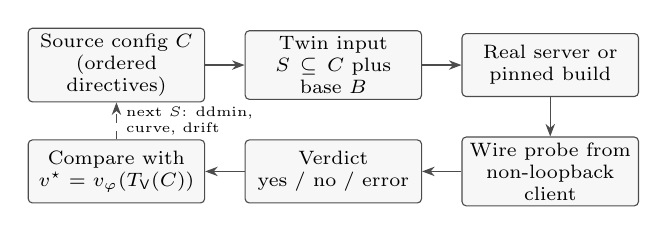
\begin{tikzpicture}[font=\scriptsize, node distance=2.5mm and 5mm,
  box/.style={draw=black!70, rounded corners=1.5pt, align=center, text width=21mm, minimum height=8mm, inner sep=2pt, fill=black!3},
  arr/.style={-{Stealth[length=1.6mm]}, draw=black!70}]
\node[box] (src) {Source config $C$\\(ordered directives)};
\node[box, right=of src] (sub) {Twin input\\$S\subseteq C$ plus base $B$};
\node[box, right=of sub] (srv) {Real server or\\pinned build};
\node[box, below=5mm of srv] (probe) {Wire probe from\\non-loopback client};
\node[box, left=of probe] (ver) {Verdict\\yes / no / error};
\node[box, left=of ver] (cmp) {Compare with\\$v^\star=v_\varphi(T_\Vb(C))$};
\draw[arr] (src) -- (sub);
\draw[arr] (sub) -- (srv);
\draw[arr] (srv) -- (probe);
\draw[arr] (probe) -- (ver);
\draw[arr] (ver) -- (cmp);
\draw[arr, dashed] (cmp) -- node[right, align=left, font=\tiny]{next $S$: ddmin,\\curve, drift} (src);
\end{tikzpicture}
\caption{Measurement loop. Every verdict comes from an unmodified server started from rendered files and probed over TCP with the stock client.}
\label{fig:loop}
\end{figure}

\subsection{Servers, scaffolding and probes}
Each evaluation writes rendered files, starts a fresh server, waits for readiness, probes it and stops it (Fig.~\ref{fig:loop}). Ports, PID files, data directories, host keys and the document tree are fixed scaffolding per worker slot, so they never become fidelity variables. The server binds to, and the client connects from, a non-loopback address; this matters because Redis protected mode treats loopback clients differently. The five properties are:
\begin{itemize}
\item \textbf{Redis}: \texttt{redis-cli CONFIG GET maxmemory} succeeds without credentials. This is an administrative command, so ACL categories and renamed commands matter.
\item \textbf{PostgreSQL}: \texttt{psql -w} as role \texttt{synthetic} runs \texttt{SELECT 1} with no password.
\item \textbf{Nginx (two)}: the \texttt{Server} header of \texttt{GET /} reveals a version; \texttt{GET /admin/} returns 200.
\item \textbf{OpenSSH}: user \texttt{synthetic} logs in with a synthetic password and runs a command.
\end{itemize}
Probes classify only recognized outcomes, such as \texttt{NOAUTH}, ``no pg\_hba.conf entry'' or ``Permission denied''. Anything else is retried once and otherwise marked inconclusive, and no inconclusive outcome survived the retry. The reference servers were the Ubuntu 24.04 builds of Redis 7.0.15, PostgreSQL 16.15, Nginx 1.24.0 and OpenSSH 9.6p1, on a 4-vCPU, 16\,GB container with four parallel worker slots. A verdict cache keyed by the canonical twin avoided repeated runs. Re-running 1,000 cached twins on fresh processes reproduced all 1,273 verdicts.

\subsection{Pinned builds}
For \RQ{5} the same renderers and probes drive 16 pinned container builds in the host network namespace, so each binds exactly the addresses a native server would. The builds are Redis 6.0, 6.2, 7.0, 7.2 and 7.4 (official images); PostgreSQL 12, 14, 16 and 17; Nginx 1.20, 1.24 and 1.27; and OpenSSH 8.8p1, 9.3p2, 9.7p1 and 10.0p2.

\subsection{Synthetic corpus and drift}
No public corpus pairs service configurations with wire-verified verdicts, so we first generated one from a seeded catalog. For each family the catalog lists legal sections, plausible values and a class label, \emph{security} or \emph{operational}. Generation combines 3--10 operational directives with a \emph{posture}, a short recipe modeled on a familiar pattern. Examples are protected mode switched off for a container network, a pg\_hba trust rule for a CI subnet, a server-wide \texttt{deny all} reopened in one location, or an appended sshd override that never takes effect. A candidate becomes a source only if the real server starts and answers conclusively; three of 360 candidates failed. The first 60 accepted configurations per family (240 in total, 5--16 directives each) form the corpus, split by index parity into training and held-out halves. The class label is used only for the expert guard set and the drift mix, never for cores or pivots.

Each held-out configuration receives three 40-edit traces in which a share $q\in\{0.1,0.3,0.5\}$ of edits target security keys. An edit modifies a directive with probability 1/2, or adds, deletes or moves one with probability 1/6 each. An edit the server refuses is rolled back, as an operator would roll it back; this happened 32 times.

\subsection{Public corpus and histories}
For \RQ{6} we used GitHub code search to collect \texttt{redis.conf}, \texttt{sshd\_config} and \texttt{pg\_hba.conf} files from public repositories, retrieving 2,363 files. A fixed pipeline turned each file into the directive model, as follows.
\begin{itemize}
\item It rejected templates and manual pages (468 files), detected by template markers and by the share of keys the server recognizes.
\item It dropped environment-bound directives a twin must supply itself: ports, sockets, file paths, includes, modules, TLS material, PAM and replication peers.
\item It remapped concrete LAN bind addresses to the twin's address and replaced every secret with the synthetic lab password.
\item It studied PostgreSQL through pg\_hba.conf, with the server listening on all addresses.
\end{itemize}
De-duplication by normalized content left 1,092 distinct configurations: 420 Redis, 339 PostgreSQL and 333 OpenSSH. For 1,500 sampled files we replayed the git history from blob-less clones. 216 files had at least two parseable versions, giving 698 versions and 426 consecutive-version commits. Nginx was excluded because real Nginx files depend on site-specific includes and upstreams that our scaffold cannot reproduce faithfully.

\subsection{Static analyzers}
For \RQ{7} we wrote two analyzers from documentation before any comparison, and did not tune them on the synthetic results. The \emph{naive} one mirrors the original platform's static baseline: it looks up the last value of a few keys. The \emph{careful} one encodes documented semantics: last-wins and first-wins keys, pg\_hba first match, Nginx per-level inheritance of access rules, sshd \texttt{Match} precedence and Redis ACL tokens. To run on public files it was extended once, before evaluation, to the full pg\_hba column syntax (netmask columns, keyword addresses and comma lists).

\subsection{Metrics}
Error rates are averaged per configuration and then across configurations. 95\% intervals come from a cluster bootstrap over configurations with 2,000 resamples. For drift we report re-emulations per 100 edits, the share of stale steps (twin verdict $\neq$ source verdict) and \emph{late flips}, meaning true verdict changes not caught at the edit that caused them.

\section{Results}\label{sec:results}

\subsection{\RQ{1}: Partial fidelity is fragile}

\begin{figure*}[t]
\centering
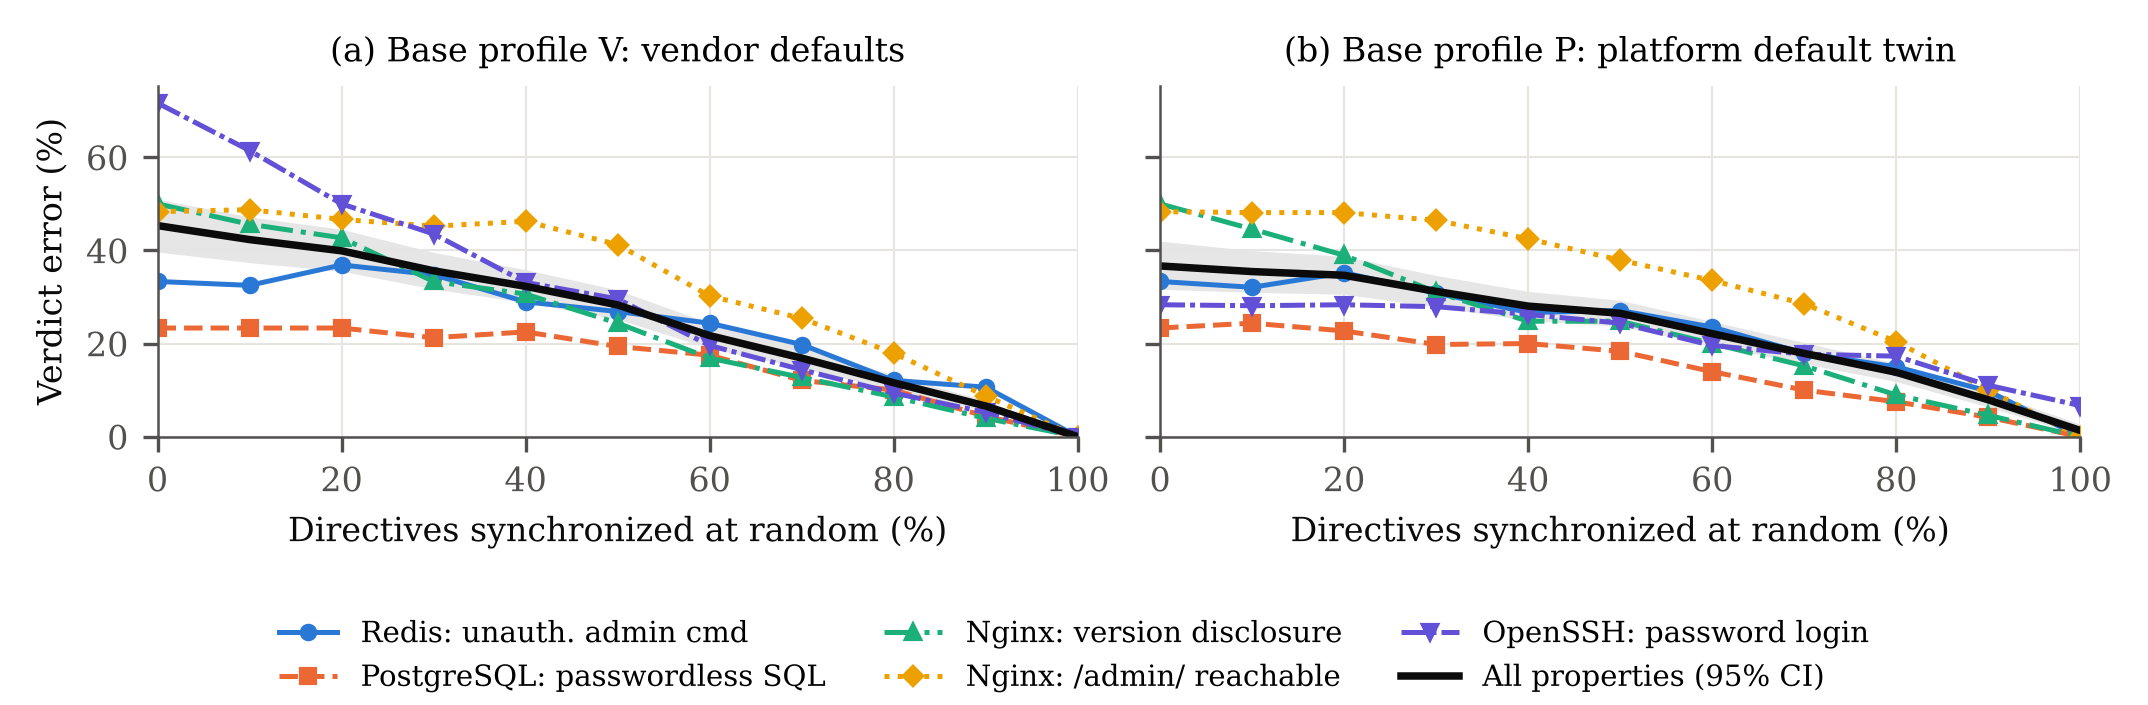
\includegraphics[width=\textwidth]{figs/fig-fidelity-curve.png}
\caption{Fidelity curves on the synthetic corpus. Verdict error of twins that mirror a random fraction of the source directives, on top of (a) vendor defaults and (b) the platform default-twin profile. Black: all properties, with a 95\% cluster-bootstrap interval.}
\label{fig:curve}
\end{figure*}

Error falls roughly linearly with the share of directives mirrored (Fig.~\ref{fig:curve}). There is no early plateau where ``most of the configuration'' is good enough. Under $\Vb$, overall synthetic error was 45.3\% with nothing mirrored, 28.3\% at half (95\% CI 25.2--31.5\%), 11.6\% at 80\% and still 6.6\% (5.5--7.8\%) at 90\%. SSH starts highest (71.7\%), because the vendor default allows password login and most sources disallow it somehow. PostgreSQL stays flat near 23\% until most rules are present, because a trust rule matters only together with \texttt{listen\_addresses} and every earlier matching rule. Public configurations show the same shape (Section~\ref{sec:rw}).

The direction of error depends on the base. Across partial levels under $\Vb$, false alarms outnumbered false-safe verdicts 3,658 to 1,980: a random cut tends to drop a defensive line and leave an exposure standing. The platform profile $\Pb$ halves the SSH error at low fidelity but never reaches zero. At full synchronization it still erred on 1.3\% of synthetic verdicts, all SSH, because sources that relied on the vendor default for \texttt{PasswordAuthentication} were overridden by the platform's ``no''. In 88 runs that value also stopped sshd from starting, because it contradicted an \texttt{AuthenticationMethods} line in the source. A base profile is not a neutral filler. It is configuration the source never had.

\subsection{\RQ{2}: Cores are tiny and usually unique, but miss pivots}

\begin{figure}[t]
\centering
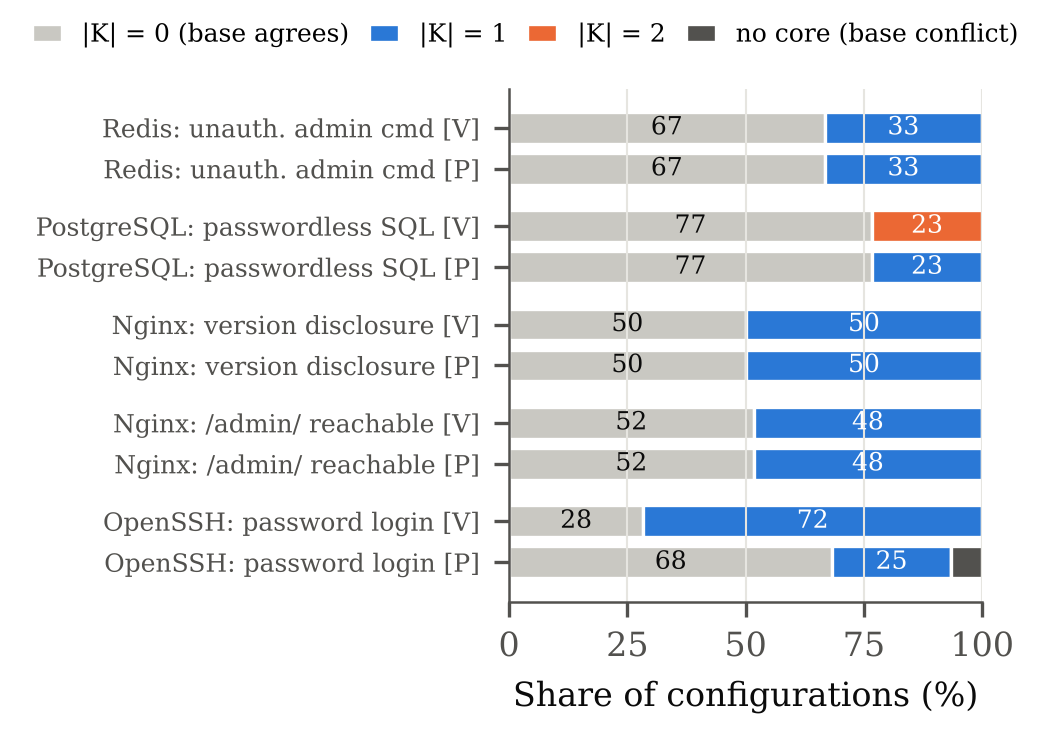
\includegraphics[width=\columnwidth]{figs/fig-core-size.png}
\caption{Fidelity-core sizes on the synthetic corpus under the vendor [V] and platform [P] bases. Gray: the base alone already reproduces the source verdict.}
\label{fig:cores}
\end{figure}

Across all 300 synthetic configuration--property pairs under $\Vb$, the largest core held two directives, the median was zero and the mean 0.50, about 5.1\% of a configuration (Fig.~\ref{fig:cores}). Size-two cores appeared only for PostgreSQL exposures, which need \texttt{listen\_addresses} and the first matching trust rule. An exhaustive search over all subsets of up to two directives confirmed that ddmin's core was a \emph{minimum} core in all 300 pairs under $\Vb$ and all 296 under $\Pb$. The minimum core was unique in 266 pairs (89\%). The other 34 had two or three equally small cores, 20 of them for SSH, where login is often blocked for several independent reasons. A core cost 3.2--5.1 server runs on average on the synthetic corpus (at most 22) and 2.6--5.6 on public files (at most 24, for files of up to 87 directives).

Small cores do not mean a small relevant set (Table~\ref{tab:cores}). Of 194 synthetic pivots, 76 (39\%) lay outside the vendor core. For Nginx \texttt{/admin/} only 22 of 62 pivots were in the core, the pattern of Fig.~\ref{fig:example}. Conversely, 79--91\% of directives labeled \emph{security} were in no vendor core, among them \texttt{PermitRootLogin}, \texttt{PubkeyAuthentication} and pg\_hba rules shadowed by an earlier match. A security label is a statement about a key. A core is a statement about one verdict. Public Redis files are more than twice as long as the synthetic ones and public sshd files somewhat longer, yet their cores were just as small. In public Redis files, 10 of 36 pivots (\texttt{requirepass}, ACL \texttt{user} lines and \texttt{rename-command}) lay outside the core. Each was a line that keeps a server with \texttt{protected-mode no} safe.

\begin{table}[t]
\caption{Cores (sufficiency) versus pivots (necessity), base $\Vb$}
\label{tab:cores}
\centering
\setlength{\tabcolsep}{2.4pt}
\footnotesize
\begin{tabular}{@{}llcccccc@{}}
\toprule
Corpus & $\varphi$ & Configs & $\overline{n}$ & $\overline{|K|}$ & max $|K|$ & Pivots & in $K$\\
\midrule
\multirow{5}{*}{Synthetic} & Redis & 60 & 9.0 & 0.33 & 1 & 43 & 20\\
 & PostgreSQL & 60 & 10.8 & 0.47 & 2 & 33 & 26\\
 & Nginx leak & 60 & 10.4 & 0.50 & 1 & 27 & 27\\
 & Nginx admin & 60 & 10.4 & 0.48 & 1 & 62 & 22\\
 & SSH & 60 & 10.2 & 0.72 & 1 & 29 & 23\\
\midrule
\multirow{3}{*}{Public} & Redis & 150 & 21.4 & 0.17 & 1 & 36 & 26\\
 & PostgreSQL & 150 & 6.7 & 0.21 & 2 & 33 & 32\\
 & SSH & 150 & 13.1 & 0.69 & 1 & 60 & 58\\
\bottomrule
\multicolumn{8}{@{}p{0.97\columnwidth}@{}}{\footnotesize $\overline{n}$: mean directives per configuration. Pivots: directives whose single removal flips the verdict; ``in $K$'': how many of those are in the ddmin core. Public: seeded sample of accepted files.}
\end{tabular}
\end{table}

\subsection{\RQ{3}: Selective synchronization and transfer}
Table~\ref{tab:gsync} evaluates twins that receive only directives whose key is in a guard set learned on the synthetic training half. Learned from cores alone, $G_{\text{core}}$ for Redis is just \texttt{protected-mode}, and held-out accuracy drops to 91.4\%: the core never ``sees'' the directives that keep a service safe. Adding pivot keys raises accuracy to 99.3\% while exporting 24\% of directives. The six remaining errors involve keys that were never decisive in the training half, Redis \texttt{bind} and sshd \texttt{DenyUsers}. These are exactly the locality failures Proposition~\ref{prop:local} anticipates for a learned guard. The expert key list was locally complete on this corpus (100\%) at an export cost of 35\%.

The same guard sets, learned only from synthetic data and applied unchanged to public configurations, transferred well. Under $\Vb$ the union guard reproduced all 450 public verdicts while exporting 23.8\% of Redis and 12.3\% of OpenSSH directives. The pg\_hba file is entirely security-relevant, so it is exported whole. Cores alone again fell short on Redis (90.7\%).

Under $\Pb$ every synthetic guard set lost about five points. The expert set's 46 errors were 26 SSH false-safe verdicts (absent \texttt{PasswordAuthentication} filled with ``no''), 16 PostgreSQL false alarms (absent \texttt{listen\_addresses} filled with ``*'') and 4 SSH start failures. On public sshd files the collision was far larger: the platform profile misjudged 22\% of them even at full synchronization (Section~\ref{sec:rw}). These are the errors Proposition~\ref{prop:silent} rules out once the agent reports absence. With absence markers, $\Pb$ becomes silent for these guard sets and the twin reduces to the $\Vb$ columns by construction.

\begin{table}[t]
\caption{Selective synchronization with learned and expert guard sets}
\label{tab:gsync}
\centering
\setlength{\tabcolsep}{2.6pt}
\footnotesize
\begin{tabular}{@{}lcccccc@{}}
\toprule
& \multicolumn{3}{c}{Synthetic held-out} & \multicolumn{3}{c}{Public, transfer ($\Vb$)}\\
\cmidrule(lr){2-4}\cmidrule(lr){5-7}
Guard set & Exp. & Acc.\ $\Vb$ & Acc.\ $\Pb$ & Redis & SSH & PG\\
\midrule
$G_{\text{core}}$ & 20.5\% & 91.4\% & 86.4\% & 90.7\% & 100\% & 100\%\\
$G_{\text{pivot}}$ & 23.8\% & 98.4\% & 93.7\% & -- & -- & --\\
$G_{\text{core}}\cup G_{\text{pivot}}$ & 24.1\% & 99.3\% & 94.3\% & 100\% & 100\% & 100\%\\
$G_{\text{expert}}$ & 34.8\% & 100\% & 94.9\% & 100\% & 100\% & 100\%\\
\midrule
\multicolumn{4}{@{}l}{Exported share, public ($G_{\text{core}}\cup G_{\text{pivot}}$)} & 23.8\% & 12.3\% & 100\%\\
\bottomrule
\multicolumn{7}{@{}p{0.97\columnwidth}@{}}{\footnotesize Synthetic: 900 held-out verdicts per row (150 pairs $\times$ 6 versions). Public: 150 configurations per family; guard sets learned on the synthetic training half and applied unchanged.}
\end{tabular}
\end{table}

\subsection{\RQ{4}: Drift and re-emulation}

\begin{figure}[t]
\centering
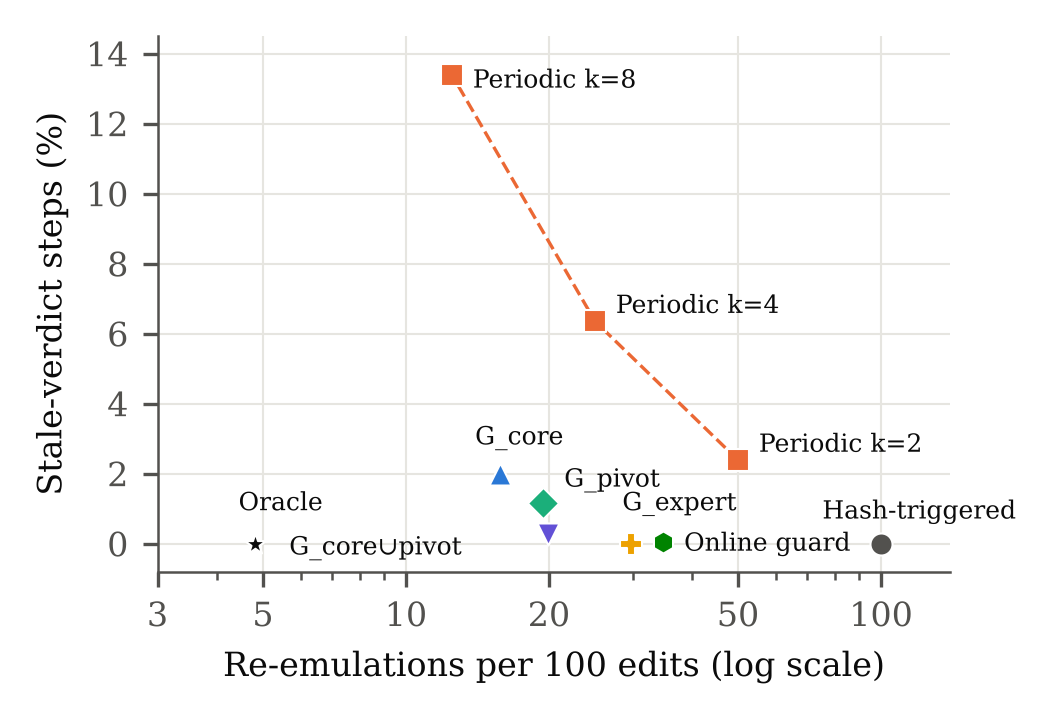
\includegraphics[width=\columnwidth]{figs/fig-resync.png}
\caption{Cost and staleness of re-emulation policies over 120 held-out synthetic drift traces of 40 edits ($q=0.3$). Lower-left is better; the oracle re-emulates only when the true verdict flips.}
\label{fig:resync}
\end{figure}

Re-emulating on every hash change is never stale, but nearly all of the work is wasted. With $q=0.3$ the true verdict flipped on only 4.8 of every 100 synthetic edits (Table~\ref{tab:resync}, Fig.~\ref{fig:resync}). Periodic re-emulation, the obvious cheap alternative, performed poorly. Every fourth edit cost 25 re-emulations per 100 edits, left 6.35\% of steps stale and caught only 93 of 289 flips at once. The learned union guard used 19.9 re-emulations per 100 edits, five times fewer than hash-triggered, with 0.28\% stale steps. It missed four flips, all of them \texttt{bind} or \texttt{DenyUsers} edits. The expert guard was never stale, at 29.7 per 100. Guards also adapt to the property: for Nginx version disclosure the learned guard is only \texttt{server\_tokens}, and it re-emulated on 6.2 of 100 edits. Audits and online guard growth cut residual staleness to 0.13\% and 0.03\%, but cost about as much as the expert list. The ordering held for $q=0.1$ and $q=0.5$. The union guard needed 6.5 and 32.2 re-emulations per 100 edits (1.05\% and 0.58\% stale), the expert guard 9.9 and 49.6 (never stale).

Real histories behave like a low-$q$ trace with bigger edits. Of 426 public commits, 180 changed only comments or environment-bound lines, 246 changed the parsed configuration, and 19 flipped a verdict: 7 Redis, 7 OpenSSH and 5 PostgreSQL. Re-emulating per commit would have cost 426 runs and per directive-hash change 246. The learned union guard needed 137 and the expert guard 159, and both caught all 19 flips at the commit that caused them.

\begin{table}[t]
\caption{Re-emulation policies (synthetic, $q=0.3$; public histories)}
\label{tab:resync}
\centering
\setlength{\tabcolsep}{3pt}
\footnotesize
\begin{tabular}{@{}lccc@{}}
\toprule
Policy & Re-emul./100 & Stale steps & Late flips\\
\midrule
\multicolumn{4}{@{}l}{\emph{Synthetic: 4,800 edits, 289 true flips}}\\
Hash-triggered (current) & 99.8 & 0.00\% & 0\\
Periodic, $k=2$ & 50.0 & 2.38\% & 143\\
Periodic, $k=4$ & 25.0 & 6.35\% & 196\\
Periodic, $k=8$ & 12.5 & 13.38\% & 221\\
Guard $G_{\text{core}}$ & 15.8 & 2.00\% & 24\\
Guard $G_{\text{pivot}}$ & 19.5 & 1.15\% & 14\\
Guard $G_{\text{core}}\cup G_{\text{pivot}}$ & 19.9 & 0.28\% & 4\\
Guard $G_{\text{expert}}$ & 29.7 & 0.00\% & 0\\
Union guard + audit every 8 & 29.8 & 0.13\% & 4\\
Online-grown guard & 34.8 & 0.03\% & 1\\
Oracle (lower bound) & 4.8 & 0.00\% & 0\\
\midrule
\multicolumn{4}{@{}l}{\emph{Public histories: 426 commits, 19 true flips}}\\
Per commit & 100 & 0.00\% & 0\\
Per directive-hash change & 57.7 & 0.00\% & 0\\
Guard $G_{\text{core}}\cup G_{\text{pivot}}$ & 32.2 & 0.00\% & 0\\
Guard $G_{\text{expert}}$ & 37.3 & 0.00\% & 0\\
Oracle (lower bound) & 4.5 & 0.00\% & 0\\
\bottomrule
\end{tabular}
\end{table}

\subsection{\RQ{5}: Versions and builds}\label{sec:versions}
Table~\ref{tab:versions} replays 120 configurations per family (60 corpus configurations and 60 drift versions) on every pinned build. For three of the four families, nothing changed. PostgreSQL 12--17, Nginx 1.20--1.27 and OpenSSH 8.8--10.0 returned the same verdict as the reference server for every configuration and property, and their core keys were identical across builds (Redis: 56 of 60). For these properties the version number is not a fidelity variable.

Redis was different in three ways, each a distinct fidelity trap:
\begin{itemize}
\item \textbf{Syntax.} Redis 6.0 refused to start on 26 configurations that use syntax introduced later: 24 ACL lines with the \texttt{\&*} channel selector and two \texttt{bind * -::*} wildcards.
\item \textbf{Semantics.} Eight configurations flipped from exposed on 6.2 to safe on 7.0. Before 7.0, an explicit \texttt{bind} disabled protected mode; from 7.0 it no longer does.
\item \textbf{Build defaults.} The official 7.0.15 container image disagreed with the Ubuntu 7.0.15 package on 11 configurations, all of which leave \texttt{protected-mode} unset. Querying each image with an empty configuration showed why: every official Redis image we tested (6.0--7.4) reports \texttt{protected-mode no} by default, while the Ubuntu build reports \texttt{yes}.
\end{itemize}
A twin pinned to ``Redis 7.0.15'' can therefore give opposite verdicts depending on where the binary came from. Version strings are a necessary fidelity check, not a sufficient one.

\begin{table}[t]
\caption{Verdict differences across pinned builds (120 configs per family)}
\label{tab:versions}
\centering
\setlength{\tabcolsep}{3pt}
\footnotesize
\begin{tabular}{@{}lccc@{}}
\toprule
Build & Start err. & Differs & Cause\\
\midrule
Redis 6.0 (image) & 26 & 40 & syntax, bind rule, default\\
Redis 6.2 (image) & 0 & 19 & bind rule, build default\\
Redis 7.0/7.2/7.4 (image) & 0 & 11 each & build default\\
PostgreSQL 12/14/16/17 & 0 & 0 & --\\
Nginx 1.20/1.24/1.27 & 0 & 0 & --\\
OpenSSH 8.8/9.3/9.7/10.0 & 0 & 0 & --\\
\bottomrule
\multicolumn{4}{@{}p{0.97\columnwidth}@{}}{\footnotesize Reference: Ubuntu 24.04 builds (Redis 7.0.15, PostgreSQL 16.15, Nginx 1.24.0, OpenSSH 9.6p1). ``Differs'': configurations whose verdict differs from the reference on any property.}
\end{tabular}
\end{table}

\subsection{\RQ{6}: Public configurations}\label{sec:rw}

\begin{figure*}[t]
\centering
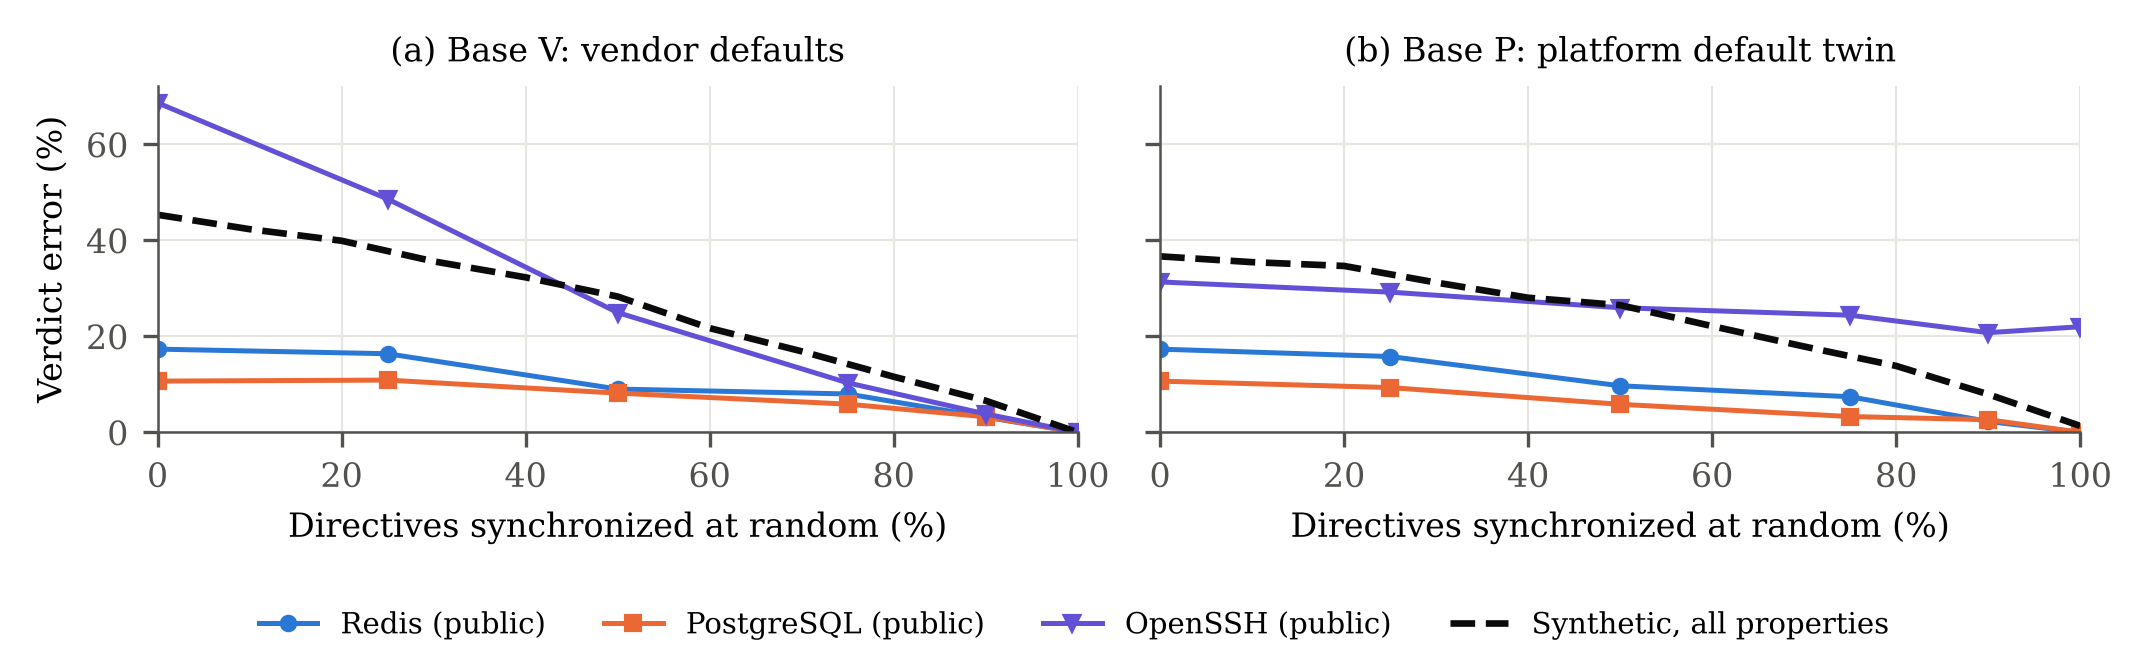
\includegraphics[width=\textwidth]{figs/fig-rw-curve.png}
\caption{Fidelity curves on public configurations (150 sampled files per family) compared with the synthetic curve. Under base P, public sshd files never reach zero error, because 22\% of them rely on the vendor default for password login.}
\label{fig:rwcurve}
\end{figure*}

\textbf{Acceptance.} Before any twin is built, a source must run. The reference servers rejected 45 of 420 public Redis files (10.7\%), mostly for directives belonging to other Redis versions. They rejected 43 of 333 sshd files (12.9\%), for invalid option combinations, options newer than OpenSSH 9.6 (such as post-quantum key-exchange names), seven configurations that never became ready, and six that require keyboard-interactive methods our PAM-less twin cannot provide. They rejected 10 of 339 pg\_hba files (3\%). These rejections are fidelity gaps in their own right: a twin pinned to the wrong release cannot even start.

\textbf{Verdicts.} Among accepted files, 72 of 375 Redis configurations (19\%) accepted unauthenticated administrative commands from a non-loopback client under the reference build's defaults. 34 of 329 pg\_hba files (10\%) let an unlisted role run SQL without a password from the twin's address, and 95 of 290 sshd files (33\%) allowed password login for an ordinary account. These figures describe the twin setting, not the deployed systems, whose network position we do not know.

\textbf{Curves and cores.} Under $\Vb$, pooled error was 32.2\% with nothing mirrored, 14.1\% at half and 3.4\% at 90\% (Fig.~\ref{fig:rwcurve}). Public Redis and PostgreSQL files start lower than the synthetic corpus because most of them are safe by default and rarely override that. Public sshd files start high and fall steeply, as in the synthetic data. Under $\Pb$ the sshd curve never reaches zero: 33 of 150 sampled sshd files (22\%) had no core at all, because the platform's \texttt{PasswordAuthentication no} contradicts files that rely on the vendor default. Cores stayed at most two directives in every family (Table~\ref{tab:cores}).

\subsection{\RQ{7}: Static analysis versus the real servers}\label{sec:static}
If only one or two directives matter, why not just read them? On the 13,606 distinct synthetic configurations, the naive analyzer was right only 72--93\% of the time (Table~\ref{tab:static}). It ignored sshd's first-value rule, pg\_hba ordering and scoping, and Nginx's rule that any access directive at an inner level replaces the parent's whole list. The careful analyzer agreed with the servers on 17,018 of 17,032 synthetic verdicts. Each of its 14 errors traced to documented behavior that is easy to read the wrong way:
\begin{itemize}
\item \textbf{Redis ACL lines rebuild the user.} The line \texttt{user default on nopass \~{}* \&* +@read +@write} produced a user who could \emph{not} run \texttt{CONFIG}. The analyzer had treated these rules as additions to the implicit \texttt{+@all}.
\item \textbf{The ACL line beats \texttt{requirepass} regardless of order.} With \texttt{user default \ldots{} nopass} earlier in the file and \texttt{requirepass} later, the server still accepted unauthenticated clients. These four errors were missed exposures.
\item \textbf{\texttt{satisfy any} needs an explicit allow.} When no access rule matched the client, the analyzer assumed the implicit allow satisfied the condition. Nginx answered 401.
\end{itemize}
On public files the careful analyzer reached 99.0--100\% (Table~\ref{tab:static}), but its six errors were of a new kind. Three Redis files defined additional ACL users, and the analyzer, written against the synthetic catalog, applied every \texttt{user} line to the default user. Two sshd files used syntax it did not model, a wildcard in \texttt{AllowGroups} and space-separated alternatives in \texttt{AuthenticationMethods}. One sshd disagreement was an artifact of our probe: a \texttt{ForceCommand} replaced the probe's command after a successful login. The pattern matters more than the count. A static model must be extended for every syntax it meets in the wild, while the twin inherits the server's own parser.

\begin{table}[t]
\caption{Static analyzers against real-server verdicts}
\label{tab:static}
\centering
\setlength{\tabcolsep}{2.6pt}
\footnotesize
\begin{tabular}{@{}lccccc@{}}
\toprule
& \multicolumn{2}{c}{Synthetic, naive} & \multicolumn{2}{c}{Synthetic, careful} & Public\\
\cmidrule(lr){2-3}\cmidrule(lr){4-5}\cmidrule(lr){6-6}
$\varphi$ & Acc. & FP / FN & Acc. & FP / FN & careful\\
\midrule
Redis unauth.\ admin & 88.4\% & 392 / 4 & 99.82\% & 2 / 4 & 99.2\%\\
PG passwordless SQL & 74.5\% & 868 / 0 & 100\% & 0 / 0 & 100\%\\
Nginx version leak & 92.7\% & 157 / 94 & 100\% & 0 / 0 & --\\
Nginx /admin/ open & 76.1\% & 127 / 691 & 99.77\% & 8 / 0 & --\\
SSH password login & 72.3\% & 843 / 90 & 100\% & 0 / 0 & 99.0\%\\
\bottomrule
\multicolumn{6}{@{}p{0.97\columnwidth}@{}}{\footnotesize Synthetic: 13,606 distinct configurations (corpus and drift versions). Public: 375 Redis, 329 PostgreSQL and 290 OpenSSH accepted files.}
\end{tabular}
\end{table}

\subsection{Cost}
The study ran about 60,000 distinct twin evaluations. On native servers the median wall time per evaluation, from start to probe to stop, was 26\,ms for Nginx, 79\,ms for PostgreSQL, 131\,ms for Redis and 161\,ms for OpenSSH. Container builds added roughly 0.3\,s, or about 2\,s for PostgreSQL. At these costs, cores, pivots and per-edit checks are practical inside a live platform rather than only in an offline study.

\section{Discussion}\label{sec:discussion}

\textbf{Design rules for twin platforms.} The results translate into five concrete rules.
\begin{enumerate}
\item \emph{Synchronize by guard keys.} Export only directives whose keys are in the union of learned and expert guard sets: a quarter of a Redis file and an eighth of an sshd file in the public corpus. This narrows what a multi-tenant control plane holds about each customer at no measured cost in accuracy.
\item \emph{Ship absence.} For every guard key the agent should report ``unset'' explicitly, so that platform defaults never stand in for vendor defaults (Proposition~\ref{prop:silent}). This was the single largest source of error we found in the public data.
\item \emph{Pin the build, not just the version.} Record where the binary came from and verify compiled defaults by querying the running twin. The Redis images showed that the same version string can carry opposite security defaults.
\item \emph{Guard re-emulation by key, with the expert list as a floor.} Key guards cut re-emulation three- to five-fold on synthetic drift and by 44\% against directive hashes on real commits, with no stale verdicts in either case for the expert guard. Learned keys can trim the list per property, but a learned guard cannot know keys that never mattered in its sample.
\item \emph{Report cores and pivots with findings.} A core is a minimal explanation (``this verdict is due to line 7''). The pivots are a remediation map (``removing line 12 would expose the service''). Both are cheap to compute on a live twin.
\end{enumerate}

\textbf{When is static analysis enough?} For four mature services, a careful analyst can encode almost everything, and our analyzer did. Its remaining disagreements cluster where documentation is easy to misread (ACL rebuilding, \texttt{satisfy any}) and where real files use syntax the model has not met. The analyzer and the twin are complements. The analyzer is instant and explainable; the twin keeps it honest, and fidelity cores tell the twin what it may safely leave out.

\textbf{Concentrated but fragile.} The paper's central observation is the pairing of tiny cores with a slowly falling fidelity curve. A random 90\% copy still misses the one line that matters about one time in fifteen on synthetic data, and one time in thirty on public files. Necessity lives in pivots, not cores. Fidelity is a property of a verdict, not of a file.

\section{Threats to Validity}
\textbf{Corpora.} The synthetic configurations are generated from postures we designed. The public corpus mitigates this, but it comes from repositories that publish configurations: Docker setups, tutorials and templates more than production fleets. Its rejection and exposure rates should not be read as population estimates. Core sizes describe both corpora, not a law.
\textbf{Normalization.} Dropping environment-bound directives, remapping bind addresses and studying pg\_hba with \texttt{listen\_addresses='*'} make public files runnable, but they also remove effects a deployed system would have, such as TLS-only listeners.
\textbf{Narrow properties.} Each property is one wire question. Richer properties, such as reachability through proxy chains or role-dependent SQL privileges, would likely produce larger cores and weaker locality.
\textbf{Single-host emulation.} Twins run as processes or host-network containers on one machine. Firewall, namespace and multi-service effects are outside this study, and our PAM-less sshd twin cannot model PAM stacks.
\textbf{Learned guards.} Guards were learned from 30 synthetic configurations per family. That they transferred perfectly to 450 public verdicts is encouraging but not a guarantee, which is one reason we recommend the expert list as a floor.
\textbf{Analyzer authorship.} The static analyzers were written by the same team, from documentation, before the comparisons. A different expert would make different mistakes, so we report the disagreements as examples of semantic corners, not as a ranking of tools.

\section{Ethics and Data Handling}
All servers ran in an isolated container against synthetic accounts and a synthetic password, and no external system was probed. Public files were obtained through GitHub code search and anonymous reads of public repositories. Raw files were kept outside the artifact. Secrets were replaced before parsing results were stored. The released data identify configurations only by content hash and contain no repository names, so no published verdict can be traced to a project. Exposure figures describe our twin setting, not the systems the files came from.

\section{Conclusion}
We asked how much configuration a security service twin needs, and the answer has two parts. To \emph{reproduce} a verdict, very little is needed: at most two directives in every case we measured, synthetic or public. To \emph{keep} reproducing it as files change and as platforms fill in defaults, a twin must track the larger set of directives whose removal would flip it. It must know when a key is absent, and it must run the same build as the source, not just the same version. Treating fidelity as verdict-relative rather than file-relative lets a twin platform export a quarter of a configuration, re-emulate a fraction as often and still agree with the real servers on every public verdict we tested. It also explains why a twin built from defaults, or from most of the file, can be confidently wrong. The harness, generator, normalized corpora, raw results and analysis scripts accompany this paper.

\begin{thebibliography}{00}
\bibitem{dtplatform} ``Digital Twin: Discovery, emulation and bounded hunting,'' source code and evaluation artifacts, GitHub repository poojarishreyas/Digital\_twin, 2026. [Online]. Available: \url{https://github.com/poojarishreyas/Digital_twin}
\bibitem{grieves2017} M. Grieves and J. Vickers, ``Digital twin: Mitigating unpredictable, undesirable emergent behavior in complex systems,'' in \emph{Transdisciplinary Perspectives on Complex Systems}, F.-J. Kahlen, S. Flumerfelt, and A. Alves, Eds. Cham, Switzerland: Springer, 2017, pp. 85--113.
\bibitem{tao2019} F. Tao, H. Zhang, A. Liu, and A. Y. C. Nee, ``Digital twin in industry: State-of-the-art,'' \emph{IEEE Trans. Ind. Informat.}, vol. 15, no. 4, pp. 2405--2415, Apr. 2019.
\bibitem{eckhart2018} M. Eckhart and A. Ekelhart, ``Towards security-aware virtual environments for digital twins,'' in \emph{Proc. 4th ACM Workshop Cyber-Physical System Security (CPSS)}, 2018, pp. 61--72.
\bibitem{eckhart2019} M. Eckhart and A. Ekelhart, ``Digital twins for cyber-physical systems security: State of the art and outlook,'' in \emph{Security and Quality in Cyber-Physical Systems Engineering}, S. Biffl, M. Eckhart, A. L\"{u}der, and E. Weippl, Eds. Cham, Switzerland: Springer, 2019, pp. 383--412.
\bibitem{dietz2020} M. Dietz and G. Pernul, ``Unleashing the digital twin's potential for ICS security,'' \emph{IEEE Security \& Privacy}, vol. 18, no. 4, pp. 20--27, 2020.
\bibitem{holmes2021} D. Holmes, M. Papathanasaki, L. Maglaras, M. A. Ferrag, S. Nepal, and H. Janicke, ``Digital twins and cyber security -- solution or challenge?'' in \emph{Proc. 6th South-East Europe Design Automation, Computer Engineering, Computer Networks and Social Media Conf. (SEEDA-CECNSM)}, 2021, pp. 1--8.
\bibitem{empl2025} P. Empl, D. Koch, M. Dietz, and G. Pernul, ``Digital twins in security operations: State of the art and future perspectives,'' \emph{ACM Comput. Surv.}, vol. 58, no. 1, Art. no. 18, 2025.
\bibitem{nasem2024} National Academies of Sciences, Engineering, and Medicine, \emph{Foundational Research Gaps and Future Directions for Digital Twins}. Washington, DC, USA: The National Academies Press, 2024.
\bibitem{crystalnet2017} H. H. Liu \emph{et al.}, ``CrystalNet: Faithfully emulating large production networks,'' in \emph{Proc. 26th ACM Symp. Operating Systems Principles (SOSP)}, 2017, pp. 599--613.
\bibitem{yamin2020} M. M. Yamin, B. Katt, and V. Gkioulos, ``Cyber ranges and security testbeds: Scenarios, functions, tools and architecture,'' \emph{Computers \& Security}, vol. 88, Art. no. 101636, Jan. 2020.
\bibitem{batfish2015} A. Fogel, S. Fung, L. Pedrosa, M. Walraed-Sullivan, R. Govindan, R. Mahajan, and T. Millstein, ``A general approach to network configuration analysis,'' in \emph{Proc. 12th USENIX Symp. Networked Systems Design and Implementation (NSDI)}, 2015, pp. 469--483.
\bibitem{minesweeper2017} R. Beckett, A. Gupta, R. Mahajan, and D. Walker, ``A general approach to network configuration verification,'' in \emph{Proc. ACM SIGCOMM}, 2017, pp. 155--168.
\bibitem{config2spec2020} R. Birkner, D. Drachsler-Cohen, L. Vanbever, and M. Vechev, ``Config2Spec: Mining network specifications from network configurations,'' in \emph{Proc. 17th USENIX Symp. Networked Systems Design and Implementation (NSDI)}, 2020, pp. 969--984.
\bibitem{ou2005} X. Ou, S. Govindavajhala, and A. W. Appel, ``MulVAL: A logic-based network security analyzer,'' in \emph{Proc. 14th USENIX Security Symp.}, 2005, pp. 113--128.
\bibitem{sheyner2002} O. Sheyner, J. Haines, S. Jha, R. Lippmann, and J. M. Wing, ``Automated generation and analysis of attack graphs,'' in \emph{Proc. IEEE Symp. Security and Privacy}, 2002, pp. 273--284.
\bibitem{yin2011} Z. Yin, X. Ma, J. Zheng, Y. Zhou, L. N. Bairavasundaram, and S. Pasupathy, ``An empirical study on configuration errors in commercial and open source systems,'' in \emph{Proc. 23rd ACM Symp. Operating Systems Principles (SOSP)}, 2011, pp. 159--172.
\bibitem{xu2015} T. Xu, L. Jin, X. Fan, Y. Zhou, S. Pasupathy, and R. Talwadker, ``Hey, you have given me too many knobs!: Understanding and dealing with over-designed configuration in system software,'' in \emph{Proc. 10th Joint Meeting European Software Engineering Conf. and ACM SIGSOFT Symp. Foundations of Software Engineering (ESEC/FSE)}, 2015, pp. 307--319.
\bibitem{peerpressure2004} H. J. Wang, J. C. Platt, Y. Chen, R. Zhang, and Y.-M. Wang, ``Automatic misconfiguration troubleshooting with PeerPressure,'' in \emph{Proc. 6th USENIX Symp. Operating Systems Design and Implementation (OSDI)}, 2004, pp. 245--258.
\bibitem{encore2014} J. Zhang, L. Renganarayana, X. Zhang, N. Ge, V. Bala, T. Xu, and Y. Zhou, ``EnCore: Exploiting system environment and correlation information for misconfiguration detection,'' in \emph{Proc. 19th Int. Conf. Architectural Support for Programming Languages and Operating Systems (ASPLOS)}, 2014, pp. 687--700.
\bibitem{pcheck2016} T. Xu, X. Jin, P. Huang, Y. Zhou, S. Lu, L. Jin, and S. Pasupathy, ``Early detection of configuration errors to reduce failure damage,'' in \emph{Proc. 12th USENIX Symp. Operating Systems Design and Implementation (OSDI)}, 2016, pp. 619--634.
\bibitem{ctest2020} X. Sun, R. Cheng, J. Chen, E. Ang, O. Legunsen, and T. Xu, ``Testing configuration changes in context to prevent production failures,'' in \emph{Proc. 14th USENIX Symp. Operating Systems Design and Implementation (OSDI)}, 2020, pp. 735--751.
\bibitem{conferr2008} L. Keller, P. Upadhyaya, and G. Candea, ``ConfErr: A tool for assessing resilience to human configuration errors,'' in \emph{Proc. IEEE/IFIP Int. Conf. Dependable Systems and Networks (DSN)}, 2008, pp. 157--166.
\bibitem{rabkin2011} A. Rabkin and R. H. Katz, ``Precomputing possible configuration error diagnoses,'' in \emph{Proc. 26th IEEE/ACM Int. Conf. Automated Software Engineering (ASE)}, 2011, pp. 193--202.
\bibitem{siegmund2012} N. Siegmund, S. S. Kolesnikov, C. K\"{a}stner, S. Apel, D. Batory, M. Rosenm\"{u}ller, and G. Saake, ``Predicting performance via automated feature-interaction detection,'' in \emph{Proc. 34th Int. Conf. Software Engineering (ICSE)}, 2012, pp. 167--177.
\bibitem{sayagh2020} M. Sayagh, N. Kerzazi, B. Adams, and F. Petrillo, ``Software configuration engineering in practice: Interviews, survey, and systematic literature review,'' \emph{IEEE Trans. Softw. Eng.}, vol. 46, no. 6, pp. 646--673, 2020.
\bibitem{rahman2019} A. Rahman, C. Parnin, and L. Williams, ``The seven sins: Security smells in infrastructure as code scripts,'' in \emph{Proc. 41st IEEE/ACM Int. Conf. Software Engineering (ICSE)}, 2019, pp. 164--175.
\bibitem{tang2015} C. Tang \emph{et al.}, ``Holistic configuration management at Facebook,'' in \emph{Proc. 25th ACM Symp. Operating Systems Principles (SOSP)}, 2015, pp. 328--343.
\bibitem{zeller2002} A. Zeller and R. Hildebrandt, ``Simplifying and isolating failure-inducing input,'' \emph{IEEE Trans. Softw. Eng.}, vol. 28, no. 2, pp. 183--200, Feb. 2002.
\bibitem{hildebrandt2000} R. Hildebrandt and A. Zeller, ``Simplifying failure-inducing input,'' in \emph{Proc. ACM SIGSOFT Int. Symp. Software Testing and Analysis (ISSTA)}, 2000, pp. 135--145.
\bibitem{hdd2006} G. Misherghi and Z. Su, ``HDD: Hierarchical delta debugging,'' in \emph{Proc. 28th Int. Conf. Software Engineering (ICSE)}, 2006, pp. 142--151.
\bibitem{hodovan2016} R. Hodov\'{a}n and \'{A}. Kiss, ``Practical improvements to the minimizing delta debugging algorithm,'' in \emph{Proc. 11th Int. Joint Conf. Software Technologies (ICSOFT-EA)}, 2016, pp. 241--248.
\bibitem{weiser1984} M. Weiser, ``Program slicing,'' \emph{IEEE Trans. Softw. Eng.}, vol. SE-10, no. 4, pp. 352--357, Jul. 1984.
\end{thebibliography}

\end{document}
